\documentclass[12pt]{article}
\usepackage[paperwidth=25cm,paperheight=17cm,margin=1.5cm]{geometry}
\usepackage[T1]{fontenc}
\usepackage[utf8]{inputenc}
\usepackage[magyar]{babel}
\usepackage{lmodern}
\usepackage{amsmath}
\usepackage{enumitem}
\usepackage{tikz}
\usetikzlibrary{arrows.meta,decorations.pathmorphing}
\usepackage{pgfplots}
\pgfplotsset{compat=1.16}

\pagestyle{empty}
\setlength{\parindent}{0pt}
\setlist[enumerate,1]{label=\textbf{\arabic*.}, leftmargin=*, itemsep=4pt, topsep=3pt}
\setlist[enumerate,2]{label=\alph*), leftmargin=2em, itemsep=1pt, topsep=1pt, parsep=0pt}

% egyenként érkező elektronok becsapódásai: #1 = próbálkozások száma, #2 = mag, #3 = felirat
\newcommand{\elektronpanel}[3]{%
  \begin{tikzpicture}
    \fill[black!4] (-1.6,0) rectangle (1.6,1.5);
    \pgfmathsetseed{#2}
    \foreach \i in {1,...,#1}{
      \pgfmathsetmacro{\x}{1.6*rand}
      \pgfmathsetmacro{\y}{1.5*rnd}
      \pgfmathsetmacro{\p}{cos(360*\x)*cos(360*\x)*exp(-\x*\x/0.8)}
      \pgfmathsetmacro{\u}{rnd}
      \ifdim \u pt < \p pt \fill (\x,\y) circle (0.45pt); \fi
    }
    \draw (-1.6,0) rectangle (1.6,1.5);
    \node[below] at (0,0) {\scriptsize #3};
  \end{tikzpicture}}

\begin{document}

\begin{center}\vspace*{-0.4cm}
  {\Large\bfseries A fény kettős természete -- gyakorló feladatok}\\[4pt]
  \fbox{\parbox{0.9\textwidth}{\centering
    $h = 6{,}63\cdot 10^{-34}~\text{J}\cdot\text{s}$, \quad
    $c = 3\cdot 10^{8}~\tfrac{\text{m}}{\text{s}}$, \quad
    $e = 1{,}6\cdot 10^{-19}~\text{C}$, \quad
    $m_e = 9{,}1\cdot 10^{-31}~\text{kg}$, \quad
    $1~\text{eV} = 1{,}6\cdot 10^{-19}~\text{J}$}}
\end{center}

\begin{minipage}[t]{0.60\linewidth}\vspace{0pt}
\begin{enumerate}
\item \textbf{Bemelegítő: a hőmérsékleti sugárzás.} Ha egy vasdarabot egyre jobban
  hevítünk, először sötétvörösen, majd narancssárgán, végül fehéren izzik. Az ábra
  három különböző hőmérsékletű test kisugárzott spektrumát mutatja.
  \begin{enumerate}
    \item Hogyan változik a hőmérséklettel a görbe csúcsának helye és a görbe alatti
      terület? Mit jelent ez a test színére és a kisugárzott teljesítményre?
    \item A csúcs helyét a Wien-féle eltolódási törvény adja meg:
      $\lambda_\text{max}\cdot T = 2{,}9\cdot 10^{-3}~\text{m}\cdot\text{K}$. Hol van a
      csúcs a Nap felszínének ($5800$~K) és egy izzólámpa wolframszálának ($2800$~K)
      sugárzásában? Miért rossz hatásfokú fényforrás az izzólámpa?
    \item A görbék alakját Planck csak azzal a feltevéssel tudta megmagyarázni, hogy a
      test az energiát $E = hf$ nagyságú adagokban (kvantumokban) sugározza ki. Mekkora
      egy $500$~nm-es fénykvantum energiája joule-ban és elektronvoltban?
  \end{enumerate}
\end{enumerate}
\end{minipage}\hfill
\begin{minipage}[t]{0.37\linewidth}\vspace{0pt}\centering
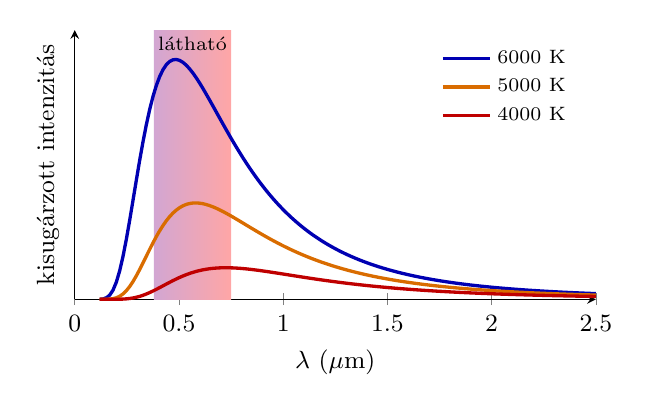
\begin{tikzpicture}
\begin{axis}[width=8.2cm,height=5.0cm,xmin=0,xmax=2.5,ymin=0,ymax=0.3,
    xlabel={$\lambda$ ($\mu$m)},ylabel={kisugárzott intenzitás},
    yticklabels={},ytick=\empty,xtick={0,0.5,1,1.5,2,2.5},
    tick label style={font=\small},label style={font=\small},
    axis lines=left,clip=false,legend style={font=\scriptsize,draw=none,fill=none,at={(0.97,0.97)},anchor=north east}]
  \fill[left color=violet!35,right color=red!35] (axis cs:0.38,0) rectangle (axis cs:0.75,0.3);
  \node[font=\scriptsize] at (axis cs:0.565,0.285) {látható};
  \addplot[very thick,blue!70!black,domain=0.12:2.5,samples=150]
    {1/(x^5*(exp(14388/(x*6000))-1))};
  \addplot[very thick,orange!85!black,domain=0.12:2.5,samples=150]
    {1/(x^5*(exp(14388/(x*5000))-1))};
  \addplot[very thick,red!75!black,domain=0.12:2.5,samples=150]
    {1/(x^5*(exp(14388/(x*4000))-1))};
  \legend{$6000$~K,$5000$~K,$4000$~K}
\end{axis}
\end{tikzpicture}
\end{minipage}

\vspace{2pt}
\begin{minipage}[t]{0.60\linewidth}\vspace{0pt}
\begin{enumerate}[start=2]
\item \textbf{A fény hullám.} Egy optikai rácsnak $1$~mm-en $500$ vonala van. Merőlegesen
  $600$~nm-es lézerfényt bocsátunk rá, az ernyő $L = 1$~m távolságban van.
  \begin{enumerate}
    \item Mekkora a rácsállandó? Mekkora szögben jelenik meg az első és a második
      elhajlási maximum, és hol látjuk őket az ernyőn?
    \item Hány fényes foltot látunk összesen (ha az ernyő elég széles)?
    \item Miért bizonyítja ez a kísérlet, hogy a fény hullám? Mi az, amit részecskékkel
      nem tudnánk megmagyarázni?
  \end{enumerate}
\end{enumerate}
\end{minipage}\hfill
\begin{minipage}[t]{0.37\linewidth}\vspace{0pt}\centering
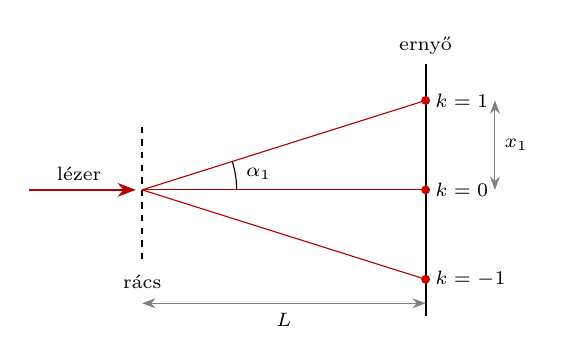
\begin{tikzpicture}[scale=0.8,>=Stealth]
  \draw[->,thick,red!70!black] (-1.8,0) -- (-0.1,0);
  \node[above,font=\scriptsize] at (-1,0) {lézer};
  \foreach \y in {-1.1,-0.9,...,1.1} \draw[thick] (0,\y) -- (0,\y+0.1);
  \node[below,font=\scriptsize] at (0,-1.2) {rács};
  \draw[thick] (4.5,-2.0) -- (4.5,2.0);
  \node[above,font=\scriptsize] at (4.5,2.0) {ernyő};
  \draw[red!70!black] (0,0) -- (4.5,0);
  \draw[red!70!black] (0,0) -- (4.5,1.42);
  \draw[red!70!black] (0,0) -- (4.5,-1.42);
  \foreach \y/\k in {0/0,1.42/1,-1.42/-1}
    \fill[red!80!black] (4.5,\y) circle (2pt) node[right,black,font=\scriptsize] {$k=\k$};
  \draw (1.5,0) arc (0:17.5:1.5);
  \node[font=\scriptsize] at (1.85,0.25) {$\alpha_1$};
  \draw[<->,gray] (5.6,0) -- node[right,font=\scriptsize,black] {$x_1$} (5.6,1.42);
  \draw[<->,gray] (0,-1.8) -- node[below,font=\scriptsize,black] {$L$} (4.5,-1.8);
\end{tikzpicture}
\end{minipage}

\newpage
\begin{minipage}[t]{0.74\linewidth}\vspace{0pt}
\begin{enumerate}[start=3]
\item \textbf{Ami nem fér bele a hullámképbe: a fényelektromos jelenség.} Egy
  elektroszkópra tiszta cinklemezt szerelünk, és negatívra töltjük (Hallwachs-kísérlet).
  \begin{enumerate}
    \item Ultraibolya lámpával megvilágítva az elektroszkóp gyorsan kisül, látható fénnyel
      viszont -- akármilyen erős lámpával -- nem. Mit jósolna a hullámelmélet? Miért
      meglepő az eredmény?
    \item A pontos mérések szerint: \textbf{(1)} van egy határfrekvencia, ami alatt nem
      lépnek ki elektronok; \textbf{(2)} a kilépő elektronok legnagyobb mozgási energiája
      csak a fény frekvenciájától függ, az intenzitásától nem; \textbf{(3)} a
      megvilágítás után azonnal (mérhető késés nélkül) megindul a kilépés. Magyarázd meg
      mindhármat azzal a feltevéssel, hogy a fény $hf$ energiájú részecskékből (fotonokból)
      áll, és egy foton egyetlen elektronnak adja át az energiáját!
    \item Írd fel Einstein fényelektromos egyenletét, és nevezd meg a tagjait!
  \end{enumerate}
\end{enumerate}
\end{minipage}\hfill
\begin{minipage}[t]{0.24\linewidth}\vspace{0pt}\centering
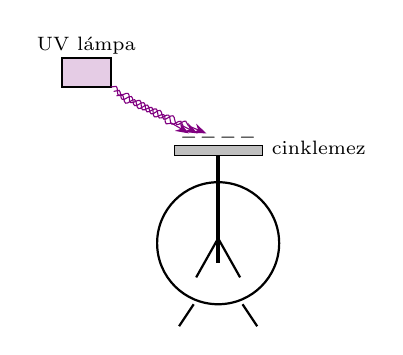
\begin{tikzpicture}[scale=0.62,>=Stealth]
  % elektroszkóp
  \draw[thick] (0,-0.2) circle (1.25);
  \draw[very thick] (0,1.6) -- (0,-0.6);
  \draw[thick] (0,-0.1) -- (-0.45,-0.9);
  \draw[thick] (0,-0.1) -- (0.45,-0.9);
  \fill[gray!50] (-0.9,1.6) rectangle (0.9,1.8);
  \draw (-0.9,1.6) rectangle (0.9,1.8);
  \node[right,font=\scriptsize] at (0.9,1.75) {cinklemez};
  \foreach \x in {-0.6,-0.2,0.2,0.6} \node[font=\scriptsize] at (\x,1.97) {$-$};
  \draw[thick] (-0.5,-1.45) -- (-0.8,-1.9);
  \draw[thick] (0.5,-1.45) -- (0.8,-1.9);
  % lámpa
  \draw[thick,fill=violet!20] (-3.2,3.0) rectangle (-2.2,3.6);
  \node[font=\scriptsize] at (-2.7,3.85) {UV lámpa};
  \foreach \d in {0,0.3,0.6}
    \draw[->,violet,decorate,decoration={snake,amplitude=1.2pt,segment length=5pt,post length=2mm}]
      (-2.2+\d*0.2,3.0-\d*0.3) -- (-0.6+\d*0.6,2.05);
\end{tikzpicture}
\end{minipage}

\vspace{2pt}
\begin{minipage}[t]{0.58\linewidth}\vspace{0pt}
\begin{enumerate}[start=4]
\item \textbf{Millikan mérése.} Egy fotocellát különböző frekvenciájú fénnyel
  világítunk meg, és mérjük azt a $U_\text{z}$ zárófeszültséget, amelynél a fotoáram
  éppen megszűnik.
  \begin{enumerate}
    \item Miért a kilépő elektronok legnagyobb mozgási energiáját méri a zárófeszültség?
    \item Ábrázold az adatokat, és illessz rájuk egyenest! Határozd meg a meredekségből
      a Planck-állandót, a tengelymetszetekből a kilépési munkát (eV-ban) és a
      határfrekvenciát! Mekkora a határhullámhossz?
    \item Mekkora a kilépő elektronok legnagyobb sebessége $400$~nm-es megvilágításnál?
    \item Hogyan változik a grafikon, ha kétszer erősebb fényt használunk? És ha egy
      nagyobb kilépési munkájú fémből készült katódot? Rajzold be!
  \end{enumerate}
\end{enumerate}
\end{minipage}\hfill
\begin{minipage}[t]{0.40\linewidth}\vspace{0pt}\centering
\renewcommand{\arraystretch}{1.2}
  \begin{tabular}{|l|c|c|c|c|c|}
  \hline
  $f$ ($10^{14}$~Hz) & $6{,}0$ & $7{,}0$ & $8{,}0$ & $9{,}0$ & $10{,}0$ \\ \hline
  $U_\text{z}$ (V)   & $0{,}19$ & $0{,}58$ & $1{,}02$ & $1{,}43$ & $1{,}83$ \\ \hline
  \end{tabular}
\\[6pt]
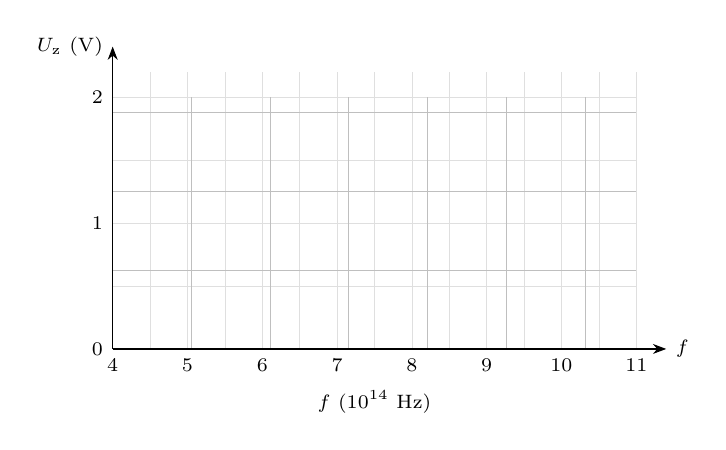
\begin{tikzpicture}[x=0.95cm,y=1.6cm,>=Stealth]
  \draw[step=0.5,gray!25,very thin] (0,0) grid (7,2.2);
  \draw[gray!50,thin] (0,0) grid (7,2);
  \draw[->] (0,0) -- (7.4,0) node[right] {\scriptsize $f$};
  \node[font=\scriptsize] at (3.5,-0.42) {$f$ ($10^{14}$ Hz)};
  \draw[->] (0,0) -- (0,2.4) node[left] {\scriptsize $U_\text{z}$ (V)};
  \foreach \x/\l in {0/4,1/5,2/6,3/7,4/8,5/9,6/10,7/11}
    \node[below,font=\scriptsize] at (\x,0) {\l};
  \foreach \y in {0,1,2}
    \node[left,font=\scriptsize] at (0,\y) {\y};
\end{tikzpicture}
\end{minipage}

\newpage
\begin{enumerate}[start=5]
\item \textbf{Akkor most részecske vagy hullám?} De Broglie szerint nemcsak a fénynek,
  hanem minden részecskének van hullámtermészete, hullámhossza $\lambda = h/p$ (a fotonra is: $p = h/\lambda = E/c$).
  \begin{enumerate}
    \item Mekkora a hullámhossza egy $100$~V feszültséggel gyorsított elektronnak? A
      kristályokban az atomok távolsága $0{,}1$--$0{,}3$~nm. Miért fontos ez az
      összehasonlítás? Miért nem lehet ugyanezt egy optikai ráccsal kimutatni?
    \item Mekkora egy $60$~g-os, $30~\tfrac{\text{m}}{\text{s}}$ sebességű teniszlabda
      hullámhossza? Miért nem tapasztaljuk a teniszlabdák elhajlását?
    \item Egy kétréses kísérletben az elektronokat \emph{egyenként} küldjük át a réseken,
      és a detektoron rögzítjük a becsapódásukat. Az ábra a felvételt mutatja egyre
      több elektron után. Mit mutat egyetlen becsapódás, és mit a sok? Hogyan
      fogalmaznád meg ebből, mit ,,jelent'' a hullám?
  \end{enumerate}
\end{enumerate}

\begin{center}
\elektronpanel{80}{11}{kb.\ 20 elektron}\hspace{0.7cm}
\elektronpanel{800}{12}{kb.\ 200 elektron}\hspace{0.7cm}
\elektronpanel{8000}{13}{kb.\ 2000 elektron}
\end{center}

\begin{enumerate}[start=6]
\item \textbf{Házi feladat -- szóbeli gyakorlás.} Fejtsd ki összefüggő szövegben, 3--4 percben: \emph{A fény
  kettős természete.} Térj ki arra, mely jelenségek mutatják a hullám-, és melyek a
  részecsketermészetet; mekkora a foton energiája és lendülete; és hogyan terjesztette ki
  de Broglie ezt a kettősséget az anyagi részecskékre!
\end{enumerate}

\end{document}
